\documentclass[11pt,a4paper]{article}
\usepackage[margin=2.3cm]{geometry}
\usepackage[T1]{fontenc}
\usepackage{lmodern}
\usepackage{amsmath,amssymb}
\usepackage{booktabs}
\usepackage{array}
\usepackage[dvipsnames]{xcolor}
\usepackage{tikz}
\usetikzlibrary{positioning,arrows.meta}
\usepackage[colorlinks=true,linkcolor=MidnightBlue,urlcolor=MidnightBlue]{hyperref}

\setlength{\parskip}{0.55em}
\setlength{\parindent}{0pt}

% Coloured boxes with plain xcolor (BasicTeX has no tcolorbox)
\newsavebox{\boxcontent}
\newcommand{\boxopen}[1]{\begin{lrbox}{\boxcontent}\begin{minipage}{\dimexpr\linewidth-14pt-0.8pt\relax}\setlength{\parskip}{0.4em}{\bfseries #1}\par}
\newenvironment{idea}[1]{\boxopen{#1}}{\end{minipage}\end{lrbox}\par\medskip\noindent{\setlength{\fboxsep}{7pt}\fcolorbox{MidnightBlue!60}{MidnightBlue!5}{\usebox{\boxcontent}}}\par\medskip}
\newenvironment{example}[1]{\boxopen{#1}}{\end{minipage}\end{lrbox}\par\medskip\noindent{\setlength{\fboxsep}{7pt}\fcolorbox{ForestGreen!60}{ForestGreen!5}{\usebox{\boxcontent}}}\par\medskip}
\newenvironment{caveat}[1]{\boxopen{#1}}{\end{minipage}\end{lrbox}\par\medskip\noindent{\setlength{\fboxsep}{7pt}\fcolorbox{BrickRed!55}{BrickRed!4}{\usebox{\boxcontent}}}\par\medskip}

\newcolumntype{L}[1]{>{\raggedright\arraybackslash}p{#1}}

\title{\textbf{How the text branch works}\\[0.3em]
\large Diary and transcript model of the Beyond-the-Clinic relapse monitor -- maths kept simple}
\author{Junction 2026 -- Aalto challenge team \\ \small (text branch built by Mahdan; this guide describes it)}
\date{14 November 2026}

\begin{document}
\maketitle

\begin{idea}{The text branch in four sentences}
The patient either writes a short diary entry or speaks a check-in that Gemini transcribes word for word.
A model trained on Reddit posts turns the text into four numbers: how much the wording resembles
depression writing, how many absolute words (``always'', ``never'') it has, how self-focused it is, and its
overall sentiment. A fixed list of crisis phrases is checked as well and goes straight to the clinician.
From then on the four numbers are treated exactly like the voice features: compared with the patient's
own healthy normal.
\end{idea}

\tableofcontents
\vspace{0.5em}

% ------------------------------------------------------------------------------------------
\section{The pipeline}

\begin{center}
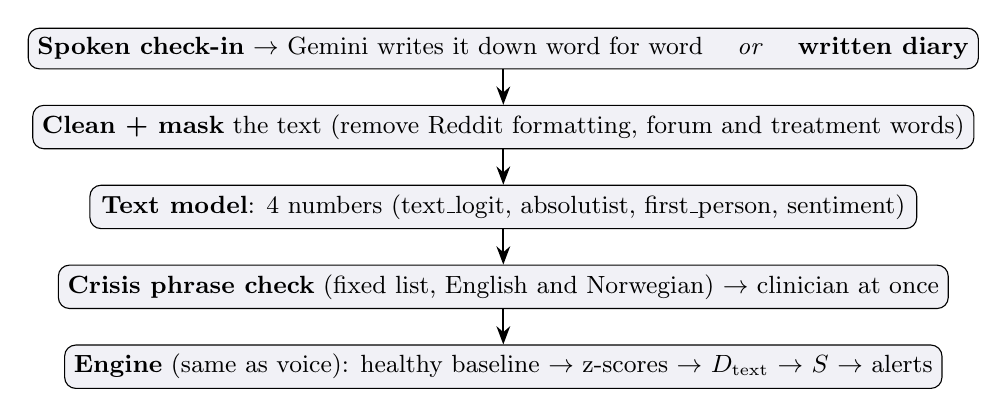
\begin{tikzpicture}[node distance=0.45cm, every node/.style={draw, rounded corners, fill=MidnightBlue!6, align=center, minimum width=10.5cm, font=\small}]
\node (a) {\textbf{Spoken check-in} $\to$ Gemini writes it down word for word \quad \emph{or} \quad \textbf{written diary}};
\node (b) [below=of a] {\textbf{Clean + mask} the text (remove Reddit formatting, forum and treatment words)};
\node (c) [below=of b] {\textbf{Text model}: 4 numbers (text\_logit, absolutist, first\_person, sentiment)};
\node (d) [below=of c] {\textbf{Crisis phrase check} (fixed list, English and Norwegian) $\to$ clinician at once};
\node (e) [below=of d] {\textbf{Engine} (same as voice): healthy baseline $\to$ z-scores $\to$ $D_{\text{text}}$ $\to$ $S$ $\to$ alerts};
\foreach \x/\y in {a/b,b/c,c/d,d/e} \draw[-{Stealth}, thick] (\x) -- (\y);
\end{tikzpicture}
\end{center}

\textbf{Transcription.} Spoken check-ins are sent to Gemini (\texttt{gemini-3.5-transcribe}) in
\emph{verbatim} mode, which keeps ``um'', repeats and false starts. The audio is sent inline and not
stored (\texttt{store=False}) and is deleted right after. The code refuses to send Androids Corpus audio.
Without an API key it falls back to a placeholder that adds nothing to the score.

% ------------------------------------------------------------------------------------------
\section{Where the training data comes from: Reddit}

The model is trained on the \textbf{Reddit Mental Health Dataset} (Low et al., 2020, \emph{Journal of
Medical Internet Research}; Zenodo record 3941387). The authors collected public Reddit posts with the
Pushshift API. The licence is the Public Domain Dedication (PDDL), but re-use is subject to Reddit's API
terms: we never commit the data and only quote short snippets.

\textbf{What is in the dataset.} Posts from 28 \emph{subreddits} (Reddit forums):
\begin{itemize}
\item 15 mental-health support groups (e.g.\ depression, anxiety, lonely, bipolarreddit, suicidewatch),
\item 2 broad ones (mentalhealth, COVID19\_support),
\item 11 non-mental-health forums (e.g.\ fitness, parenting, personalfinance, relationships, divorce).
\end{itemize}
Each file is one subreddit in one time window, \texttt{<subreddit>\_<window>\_features\_tfidf\_256.csv}.
It holds the post text, an anonymous author name, the date, and about 350 precomputed columns
(readability, sentiment, word counts, 256 TF-IDF values). \textbf{We only use the author name and the post
text}; all features are recomputed on our own text pieces, with the app's own code.

\textbf{What we use: 8 subreddits.}
\begin{center}
\small
\begin{tabular}{@{}L{5.2cm}rL{6.4cm}@{}}
\toprule
\textbf{Subreddit} & \textbf{Posts (50+ words)} & \textbf{Role}\\
\midrule
depression & 17\,545 & positive class (``depression writing'')\\
fitness, parenting, personalfinance, meditation, teaching & 64\,637 & everyday writing\\
relationships, divorce & 20\,702 & \emph{hard negatives}: emotional, but not depression\\
\bottomrule
\end{tabular}
\end{center}
The hard negatives matter: without them the model could learn ``emotional = depressed''. With them it
has to learn what is specific to depression writing.

% ------------------------------------------------------------------------------------------
\section{Before vs during COVID-19: why the ``pre'' window}

The dataset comes in four time windows:

\begin{center}
\small
\begin{tabular}{@{}lL{4.6cm}L{7.2cm}@{}}
\toprule
\textbf{Window} & \textbf{Dates} & \textbf{Purpose in the original study}\\
\midrule
\textbf{pre} & \textbf{December 2018 -- December 2019} & a full year before the pandemic (\textbf{we use this})\\
post & 1 January -- 20 April 2020 & the start of the COVID-19 pandemic\\
2019 & 1 January -- 20 April 2019 & same months one year earlier (seasonal control; overlaps ``pre'')\\
2018 & 1 January -- 20 April 2018 & same months two years earlier (seasonal control)\\
\bottomrule
\end{tabular}
\end{center}

The original paper is titled \emph{``Natural Language Processing Reveals Vulnerable Mental Health Support
Groups and Heightened Health Anxiety on Reddit During COVID-19''}: during the pandemic, what people wrote
about \emph{changed}.

\begin{idea}{Why we train on ``pre'' and not ``post''}
\begin{itemize}
\item \textbf{Topic shift.} In early 2020 many posts in every forum were about lockdown, the virus, job
      loss and health worries. A model trained on that period could learn ``pandemic words = depression''.
      A TMS patient in 2026 writing about a cold or a vaccine would then look depressed for the wrong reason.
\item \textbf{Different kind of distress.} Pandemic distress (health anxiety, isolation forced by
      lockdown) is real, but it is not the same as the depression a relapse after TMS looks like.
\item \textbf{A full year.} ``pre'' covers all seasons (winter low mood, summer, holidays), whereas
      ``post'' covers only four months.
\end{itemize}
\end{idea}

\begin{caveat}{What ``pre'' does not solve}
The text is from 2018--2019. Language moves on: words the model never saw (new slang, ``long covid'')
simply have no weight and are ignored. That is safe, but it means newer expressions of low mood are
missed. Reddit users are also not TMS patients: they chose to post in public forums, and are likely
younger and more often English-speaking North Americans.
\end{caveat}

% ------------------------------------------------------------------------------------------
\section{Preparing the text}

\begin{enumerate}
\item \textbf{Clean.} Remove links, Reddit references (``r/\dots'', ``u/\dots'') and Reddit formatting a
      diary never has (``tl;dr'', ``edit:'', age/gender tags such as ``(24/f)'').
\item \textbf{Mask.} Replace words that would give the answer away with a break that no word pair can
      cross:
      \begin{itemize}
      \item forum names: ``depress\dots'', ``subreddit'', ``meditat\dots'', ``divorc\dots'', \dots
            (otherwise the model just learns to read the forum name),
      \item treatment words: therapy, meds, doctor, symptoms, TMS, ECT, antidepressant names.
            TMS patients mention treatment on good days too, so ``mentions treatment'' must not mean
            ``depressed''.
      \end{itemize}
\item \textbf{Cut into diary-sized pieces.} Posts are cut into chunks of 50--100 words (at most 3 per
      post), so training text looks like a short diary entry.
\item \textbf{Split by author}: 70\% of the \emph{people} for training, 15\% for tuning, 15\% for the
      final test. Nobody appears in two parts, so the test measures new people, not memorised writers.
\item \textbf{Balance}: as many ``other'' as ``depression'' pieces in each part (1:1).
\end{enumerate}

% ------------------------------------------------------------------------------------------
\section{The main number: \texttt{text\_logit}}

\subsection*{Step 1 -- turn words into numbers (TF-IDF)}
For every word and every pair of neighbouring words (``word pairs'') in a text:
\[
\text{tfidf}(\text{word}) \;=\; \underbrace{\bigl(1+\log(\text{count in this text})\bigr)}_{\text{TF: how often here}}
\;\times\; \underbrace{\text{idf}(\text{word})}_{\text{IDF: how rare overall}}
\]
then all values of the text are scaled so the list has length 1. Common words (``the'', ``and'') have a
small IDF and count little; rarer, telling words count more. The vocabulary is the 50\,000 most frequent
words and word pairs that appear in at least 5 training pieces.

\subsection*{Step 2 -- weigh the words (logistic regression)}
Each word has a learned weight. The model adds them up:
\[
\text{text\_logit} \;=\; b \;+\; \sum_{\text{words in the text}} \text{weight}(\text{word}) \times \text{tfidf}(\text{word})
\]
\[
P(\text{depression-like}) \;=\; \frac{1}{1+e^{-\text{text\_logit}}}
\]
\begin{itemize}
\item \textbf{Positive weight} = pushes towards depression writing; \textbf{negative} = away from it.
\item \texttt{text\_logit} is the \emph{log-odds}: 0 means 50/50, $+2$ means odds of about 7 to 1,
      $-2$ about 1 to 7.
\end{itemize}

\begin{center}
\small
\begin{tabular}{@{}lr@{\qquad}lr@{}}
\toprule
\textbf{Towards depression} & \textbf{weight} & \textbf{Away from depression} & \textbf{weight}\\
\midrule
suicide & $+9.2$ & kids & $-7.7$\\
life & $+8.3$ & credit & $-6.6$\\
myself & $+7.0$ & he & $-6.5$\\
worse & $+6.0$ & we & $-6.0$\\
alone & $+4.1$ & workout & $-5.9$\\
nothing & $+4.6$ & gym & $-5.7$\\
anymore & $+4.2$ & son & $-5.7$\\
\bottomrule
\end{tabular}
\end{center}
The pattern: \textbf{self-focused, feelings-focused, hopeless} writing pulls up; writing about
\textbf{other people and activities} pulls down.

\begin{example}{Illustration (rounded, simplified numbers)}
A 60-word diary contains ``alone'', ``nothing'' and ``myself'' once each, and no strongly negative words.
Suppose each gets a TF-IDF value of about $0.12$. Their part of the sum is
$0.12\times(4.1+4.6+7.0) \approx +1.9$. Other words and the starting value $b$ add or subtract a bit.
If the total is $\text{text\_logit}=+1.5$, then $P = 1/(1+e^{-1.5}) \approx 0.82$.
The app can list exactly these words as the reason.
\end{example}

\textbf{Why the engine uses \texttt{text\_logit} and not $P$.} Personal diary text often scores close to 1
on the probability scale, where differences become invisible (0.97 vs 0.99). The log-odds keep those
differences, so ``more depression-like than \emph{your} normal'' is still measurable.

% ------------------------------------------------------------------------------------------
\section{Three simple extra numbers (word lists)}

\begin{center}
\small
\begin{tabular}{@{}lL{6.0cm}lcc@{}}
\toprule
\textbf{Feature} & \textbf{What} & \textbf{Worse} & \textbf{Other} & \textbf{Depression}\\
\midrule
\texttt{absolutist} & absolute words per 100 words (always, never, nothing, completely), skipping a word right after ``not'' & higher & 1.03 & 1.77\\
\texttt{first\_person} & I, me, my, mine, myself per 100 words & higher & 8.19 & 11.94\\
\texttt{sentiment} & VADER mood score from $-1$ (negative) to $+1$ (positive) & lower & 0.23 & $-0.14$\\
\bottomrule
\end{tabular}
\end{center}
The last two columns are averages on the Reddit test set. On their own the three reach AUC 0.79.
Added to \texttt{text\_logit} they give \textbf{no extra accuracy} (0.970 vs 0.970), because the main
model already uses the same words. They are kept because they are \textbf{easy to explain} to a clinician.

% ------------------------------------------------------------------------------------------
\section{The crisis check}

A fixed list of phrases is searched in every text, independent of any model, for example:
\emph{suicid\dots, kill myself, end my life, want to die, better off dead, hurt myself, can't go on},
and in Norwegian \emph{selvmord\dots, ta livet av meg, vil dø, vil ikke leve, skade meg selv}.
A match sets the crisis flag, which alerts the clinician immediately.

It does not understand negation or quotes (``I'm \emph{not} suicidal'', a news story about suicide).
That gives false crisis alerts rather than missed ones -- the safe direction -- but the clinician should
know.

% ------------------------------------------------------------------------------------------
\section{How the text enters the score}

From here the text branch uses the same engine as the voice (see the main guide, \texttt{model.pdf}):
\begin{enumerate}
\item The first weeks build the patient's \textbf{healthy baseline} for the four numbers (median and
      spread). There is no corpus spread for text, so it needs at least 5 diary entries.
\item Every new text gets z-scores: how far from the patient's own normal, in the worse direction.
\item The z-scores are weighted into $D_{\text{text}}$. The weights come from the classifier:
      \texttt{text\_logit} 0.95, the other three about 0.03 or less. In practice
      $D_{\text{text}}\approx$ ``how much more depression-like today's text is than \emph{your} normal''.
\item If voice and text exist on the same day, the day's $D$ is their average; then the smoothing $S$ and
      the alerts follow as for the voice.
\end{enumerate}

% ------------------------------------------------------------------------------------------
\section{How good is it?}

\begin{center}
\small
\begin{tabular}{@{}L{6.3cm}L{8.2cm}@{}}
\toprule
\textbf{Test} & \textbf{Result}\\
\midrule
Reddit, people never seen in training & AUC \textbf{0.970}, F1 0.908 (guessing: 0.5 / 0.667)\\
Without masking (not used) & AUC 0.977 -- masking costs little\\
False ``depression'' flags per forum & fitness 2.7\%, personal finance 2.1\%, parenting 5.7\%, relationships 13.6\%, divorce 17.3\%, \textbf{meditation 27\%}\\
10 team-written diaries & 9 of 10 right; a low day scored above its good day in 23 of 25 pairs\\
Diaries read aloud, then transcribed & average score change 0.016; no text changed side\\
Kasper's and Mahdan's own recordings & both bad days above both good days for each speaker (0.02--0.07 vs 0.53--0.73)\\
\bottomrule
\end{tabular}
\end{center}

\begin{caveat}{Why 0.97 cannot be compared with the voice model's 0.77}
The text test separates r/depression posts from other forums. Much of that difference is
\emph{genre} -- personal, feelings-focused writing -- not only mood (a good day written as ``feel more like
myself again'' scored 0.95). The voice test separates clinically diagnosed people from healthy people.
The useful signal for us is \textbf{change against the person's own baseline}, which is how the engine
uses both.
\end{caveat}

% ------------------------------------------------------------------------------------------
\section{Limitations -- said plainly}
\begin{enumerate}
\item \textbf{Genre, not only mood} (box above).
\item \textbf{Style gap in the diary test.} The good test diaries hardly use ``I'' (0--3 per 100 words),
      the low ones a lot (15--19). \texttt{first\_person} alone separates them perfectly, so the test
      partly measures ``writes about oneself''.
\item \textbf{Hidden low mood.} ``I'm fine, it's okay'' reads as positive to the sentiment score.
\item \textbf{Reddit is not a diary}, and Reddit users are not TMS patients.
\item \textbf{Old text (2018--2019).} Newer words are ignored.
\item \textbf{English only.} A Norwegian diary needs a Norwegian model or translation first (the crisis
      check does have Norwegian phrases).
\item \textbf{Personal baseline only.} No corpus spread for text; the relapse shift for text (1.5) is a
      rough estimate from 15 diaries.
\item \textbf{Not validated on relapse after TMS}, like the voice model.
\end{enumerate}

\textbf{In one sentence:} a strong, transparent text classifier that partly measures writing style; in the
app it is used the right way -- as change against the patient's own normal, alongside the voice.

% ------------------------------------------------------------------------------------------
\section*{Glossary}
\begin{description}
\item[Subreddit] a Reddit forum on one topic, written ``r/name''.
\item[Hard negative] training text that is emotional but not depression, to stop ``emotional = depressed''.
\item[Masking] replacing give-away words so the model must learn from the rest.
\item[TF-IDF] word importance: often in this text (TF) and rare overall (IDF).
\item[Logistic regression] adds weighted word values and turns the sum into a probability.
\item[Log-odds (logit)] $\log\bigl(P/(1-P)\bigr)$; 0 = 50/50, each $+1$ multiplies the odds by about 2.7.
\item[VADER] a word-list based sentiment score for short social-media text.
\item[AUC] chance that a random depression text scores above a random other text (0.5 = guessing).
\item[F1] balance of catching depression texts and not flagging others (1 = perfect).
\end{description}

\end{document}
